Bi-intuitionistic logic (BINT) is a conservative extension of
intuitionistic logic with a duality.  That is, BINT contains the
usual intuitionistic logical connectives such as true, conjunction,
and implication, but also their duals false, disjunction, and
coimplication.  One leading question with respect to BINT is, what does
BINT look like across the three arcs -- logic, typed
$\lambda$-calculi, and category theory -- of the Curry-Howard-Lambek
correspondence?  A non-trivial (does not degenerate to a poset)
categorical model of BINT is currently an open problem.  This paper
directly contributes to the solution of this open problem by giving a
new categorical model based on adjunctions for cointuitionistic logic,
and then proposing a new categorical model for BINT.  

BINT can be seen as a mixing of two worlds: the first being
intuitionistic logic (IL), which is modeled categorically by a
cartesian closed category (CCC), and the second being the dual to
intuitionistic logic called cointuitionistic logic (coIL), which is
modeled by a cocartesian coclosed category (coCCC).  Crolard
\cite{Crolard:2001} showed that combining these two categories into
the same category results in it degenerating to a poset, i.e.
there is at most one morphism between any two objects; we review this
result in
Section~\ref{subsec:cartesian_closed_and_cocartesian_coclosed_categories}.
However, this degeneration does not occur when both logics are linear.

Notice that atoms are not dualized, at least  in the main stream tradition of BINT
started by C.Rauszer \cite{Rauszer:1974, Rauszer:1980}. For this reason
T.Crolard \cite{Crolard:2001} p. 160, describes the relation between IL and coIL
within BINT as ``pseudo duality''. A duality on atoms could be added 
and this has been attemptedr with linguistic motivations \cite{Bellin:2014} 
(see the section on Related Work).
This avoids the collapse but yields a different framework.
Here we are concerned mainly with the main stream tradition.

We propose that IL and coIL need to be separated, and then mixed in a
controlled way using the modalities from linear logic.  This
separation can be ultimately achieved by an adjoint formalization of
bi-intuitionistic logic.  This formalization consists of three worlds
instead of two: the first is intuitionistic logic, the second is
linear bi-intuitionistic (Bi-ILL), and the third is cointuitionistic
logic.  They are then related via two adjunctions as depicted by the
following diagram:
\begin{center}
  \begin{tikzpicture}
    \node (img) {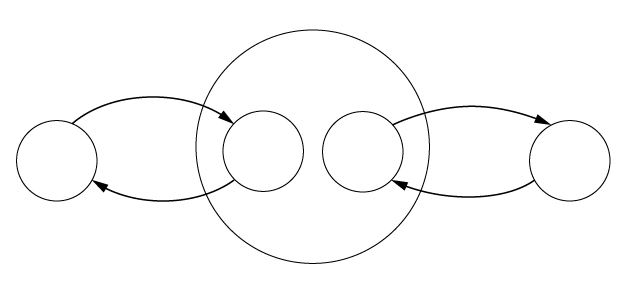
\includegraphics[scale=0.4]{introDiag}};
    \node (dv) at (-2.3, 0.0) {\huge $\dashv$};
    \node (IL) at (-3.58, -0.1) {IL};
    \node (vd) at (2.3, 0.0) {\huge $\dashv$};
    \node (coIL) at (3.65, -0.1) {coIL};

    \node (ILL) at (-0.67, 0.0) {ILL};
    \node (coILL) at (0.71, 0.0) {coILL};
    \node (BiILL) at (0, 1.0) {Bi-ILL};
  \end{tikzpicture}
    
\end{center}
The adjunction between IL and ILL is known as a Linear/Non-linear model
(LNL model) of ILL, and is due to Benton \cite{Benton:1994}.  However,
the dual to LNL models which would amount to the adjunction between coILL
and coIL has yet to appear in the literature.

Suppose $(\cat{I}, 1, \times, \to)$ is a cartesian closed category,
and $(\cat{L}, \top, \otimes, \limp)$ is a symmetric monoidal closed
category.  Then relate these two categories with a symmetric monoidal
adjunction $\cat{I} : \func{F} \dashv \func{G} : \cat{L}$
(Definition~\ref{def:SMCADJ}), where $\func{F}$ and $\func{G}$ are
symmetric monoidal functors.  The later point implies that there are
natural transformations $\m{X,Y} : \func{F}X \otimes \func{F}Y \mto
\func{F}(X \times Y)$ and $\n{A,B} : \func{G}A \times \func{G}B \mto
\func{G}(A \otimes B)$, and maps $\m\top : \top \mto \func{F}1$ and
$\n1 : 1 \mto \func{G}\top$ subject to several coherence conditions;
see Definition~\ref{def:SMCFUN}.  Furthermore, the functor $\func{F}$
is strong which means that $\m{X,Y}$ and $\m{\top}$ are isomorphisms.
This setup turns out to be one of the most beautiful models of
intuitionistic linear logic called a LNL model due to Benton
\cite{Benton:1994}.  In fact, the linear modality of-course can be
defined by $!A = \func{F}(\func{G}(A))$ which defines a symmetric
monoidal comonad using the adjunction; see Section~2.2 of
\cite{Benton:1994}.  This model is much simpler than other known
models, and resulted in a logic called LNL logic which supports mixing
intuitionistic logic with linear logic.  The main contribution of this
paper is the definition and study of the dual to Benton's LNL models
as models of cointuitionistic logic.

Taking the dual of the previous model results in what we call dual LNL
models. They consist of a cocartesian coclosed category, $(\cat{C}, 0,
+, -)$ where $- : \cat{C} \times \cat{C} \mto \cat{C}$ is left adjoint
to the coproduct, a symmetric monoidal coclosed category
(Definition~\ref{def:SMCCC}), $(\cat{L}', \perp, \oplus, \colimp)$,
where $\colimp : \cat{L}' \times \cat{L}' \mto \cat{L}'$ is left
adjoint to cotensor (usually called \emph{par}), and a symmetric
comonoidal adjunction (Definition~\ref{def:coSMCADJ}) $\cat{L'} :
\func{H} \dashv \func{J} : \cat{C}$, where $\func{H}$ and $\func{J}$
are symmetric comonoidal functors. Dual to the above, this implies
that there are natural transformations $\m{X,Y} : \func{J}(X + Y) \mto
\func{J}X \oplus \func{J}Y$ and $\n{A,B} : \func{H}(A \oplus B) \mto
\func{H}A + \func{H}B$, and maps $\m0 : \func{J}0 \mto \perp$ and
$\n\perp : \func{H}\perp \mto 0$ subject to several coherence conditions;
see Definition~\ref{def:coSMCFUN}.  In fact, one can define Girard's
exponential why-not by $\wn A = \func{JH}A$, and hence, is the monad
induced by the adjunction.

Bellin \cite{Bellin:2012} was the first to propose the dual to
Bierman's \cite{Bierman:1994} linear categories which he names dual
linear categories as a model of cointuitionistic linear logic.  We
conduct a similar analysis to that of Benton for dual LNL models by
showing that dual LNL models are dual linear categories
(Section~\ref{subsec:dual_lnl_model_implies_dual_category}), and that
from a dual linear category we may obtain a dual LNL model
(Section~\ref{subsec:dual_category_implies_dual_lnl_model}).
Following this we give the definition of bi-LNL models by combining
our dual LNL models with Benton's LNL models to obtain a categorical
model of bi-intuitionistic logic
(Section~\ref{subsec:a_mixed_bi-linear_non-linear_model}), but we
leave its analysis and corresponding logic to a future paper.

Benton~\cite{Benton:1994} showed that, syntactically, LNL models have
a corresponding logic by first defining intuitionistic logic, whose
sequent is denoted, $\Theta \vdash_{\cat{C}} X$, and then
intuitionistic linear logic, $\Theta;\Gamma \vdash_{\cat{L}} A$, but
the key insight was that $\Theta$ contains non-linear assumptions
while $\Gamma$ contains linear assumptions, but one should view their
separation as merely cosmetic; all assumptions can consistently be
mixed within a single context.  The two logics are then connected by
syntactic versions of the functors $\func{F}$ and $\func{G}$ which
allow formulas to move between both fragments.

Following Benton's lead the design of dual LNL logic is similar.  We
have a non-linear cointuitionistic fragment, $T \vdash_{\cat{C}}
\Psi$, and a linear cointuitionistic fragment, $A \vdash_{\cat{C}}
\Delta;\Psi$, where $\Delta$ contains linear conclusions and $\Psi$
contains non-linear conclusions, but again the separation of contexts
is only cosmetic. The non-linear fragment has the following structural rules:
\begin{mathpar}
  \DualLNLLogicdruleCXXwk{}  
  \and
  \DualLNLLogicdruleCXXcr{} 
\end{mathpar}
Then we connect these two fragments together using the following rules
for the functors $\func{H}$ and $\func{J}$:
\begin{mathpar}
  \DualLNLLogicdruleCXXhL{}
  \and
  \DualLNLLogicdruleLXXhR{}
  \and
  \DualLNLLogicdruleLXXjL{}
  \and
  \DualLNLLogicdruleLXXjR{}
\end{mathpar}
These allow for linear and non-linear formulas to move from one
fragment to the other.  We will give a sequent calculus and natural
deduction formalization (Section~\ref{sec:sequent_calculus} and
Section~\ref{sec:sequent-style_natural_deduction}) as well as a term
assignment (Section~\ref{sec:term_assignment}).  The latter is
particularly interesting, because of the fact that cointuitionistic
logic has multiple conclusions, but only a single hypothesis.

%%% Local Variables: 
%%% mode: latex
%%% TeX-master: main.tex
%%% End: 
